% =========================================================================
% IEEE Conference Paper – Pivot Point Identification via IMU
% Based on: Pivot_IMU.tex (Nguyen Quang The Son, HUST)
% Template: IEEEtran, two-column, conference, 6 pages
% =========================================================================
\documentclass[conference]{IEEEtran}

\usepackage[T1]{fontenc}
\usepackage[utf8]{inputenc}
\usepackage{amsmath,amssymb,amsfonts}
\usepackage{graphicx}
\usepackage{booktabs}
\usepackage{multirow}
\usepackage{siunitx}
\usepackage{cite}
\usepackage{float}
\usepackage{bm}
\usepackage{xcolor}
\usepackage[hidelinks]{hyperref}

% Figure path
\graphicspath{{../hinhanh_VT/}}

% Convenience macros
\newcommand{\vv}[1]{\bm{#1}}          % vector bold
\newcommand{\mm}{\,\text{mm}}
\newcommand{\rPH}{\vv{r}_{PH}}
\newcommand{\rPI}{\vv{r}_{PI}}
\newcommand{\omg}{\bm{\omega}}
\newcommand{\alp}{\bm{\alpha}}
\newcommand{\aH}{\vv{a}_{H}}

\IEEEoverridecommandlockouts

% =========================================================================
\begin{document}

\title{%
  IMU-Based Pivot Point and Head Position Identification\\
  for a 6-RUS Gough--Stewart Motion Simulator%
}

\author{%
  \IEEEauthorblockN{Nguyen Quang The Son}
  \IEEEauthorblockA{%
    \textit{School of Mechanical Engineering}\\
    \textit{Hanoi University of Science and Technology}\\
    Hanoi, Vietnam\\
    Son.nqt226226@sis.hust.edu.vn}
  \and
  \IEEEauthorblockN{Pham Duc An}
  \IEEEauthorblockA{%
    \textit{School of Mechanical Engineering}\\
    \textit{Hanoi University of Science and Technology}\\
    Hanoi, Vietnam}
}

\maketitle

% -------------------------------------------------------------------------
\begin{abstract}
Accurate knowledge of the relative position between the rotation center
(Pivot Point $P$) and the driver's head ($H$) is essential for
high-fidelity motion cueing on driving simulators based on the
Gough--Stewart parallel mechanism.
This paper proposes an experimental method that uses a single
inertial measurement unit (IMU) mounted at the head position to
identify the vector $\rPH$ through rigid-body kinematics and a
least-squares solver.
Roll and pitch sinusoidal maneuvers are applied on the CKAS W2 6-RUS
platform; the raw IMU data are pre-processed with a Butterworth
low-pass filter and a PCA-based axis-alignment correction before being
fed into the solver.
Experiments over six \texttt{centre\_z} settings
($0$ to $-500\mm$) yield a consistent $Z$-component
$r_{zH} = 813.6 \pm 28.6\mm$ (relative error $3.52\,\%$) with
Pearson correlation coefficients $r \ge 0.97$ and RMSE $\le
0.076\,\text{m/s}^2$ across all configurations.
The identified position is consistent with the anthropometric head
height, demonstrating the reliability of the proposed low-cost approach.
\end{abstract}

\begin{IEEEkeywords}
  motion simulator, pivot point, IMU, least squares,
  Gough--Stewart platform, CKAS W2, PCA, motion cueing
\end{IEEEkeywords}

% =========================================================================
\section{Introduction}
\label{sec:intro}

Gough--Stewart platforms \cite{Stewart1965,Gough1956} are widely used
in driving and flight simulation to reproduce 6-DOF inertial cues.
The CKAS W2, a 6-RUS variant, controls the center of rotation through
the \texttt{\textasciitilde{}centre\_z} command, which shifts the
Pivot Point $P$ along the vertical axis of the platform.
When $P$ coincides with the driver's head center $H$, angular
maneuvers produce no net linear displacement at $H$, eliminating
unwanted translational false cues and improving vestibular fidelity
\cite{Kolasinski1995}.

Identifying the correct \texttt{centre\_z} value requires knowing
$\rPH$ precisely, yet this distance depends on seat compression, posture,
and individual anthropometry — factors that are hard to measure by
mechanical means alone.
Existing work has addressed head position estimation through
motion-capture systems \cite{Draper2001} and inertial integration
\cite{Kalman1960}, but a direct IMU-based algebraic identification
exploiting the rigid-body acceleration relation has not been reported for
commercial driving simulators.

This paper makes the following contributions:
\begin{enumerate}
  \item A closed-form kinematic model relating IMU acceleration at $H$
        to the unknown vector $\rPH$ and the measured angular kinematics
        at $P$.
  \item A practical pre-processing pipeline (LPF + PCA alignment +
        time synchronisation) validated on real CKAS W2 data.
  \item Experimental identification of $\rPH$ over six pivot settings
        with statistical validation (RMSE, Pearson $r$).
\end{enumerate}

% =========================================================================
\section{System Description and Coordinate Frames}
\label{sec:system}

\begin{figure}[!t]
  \centering
  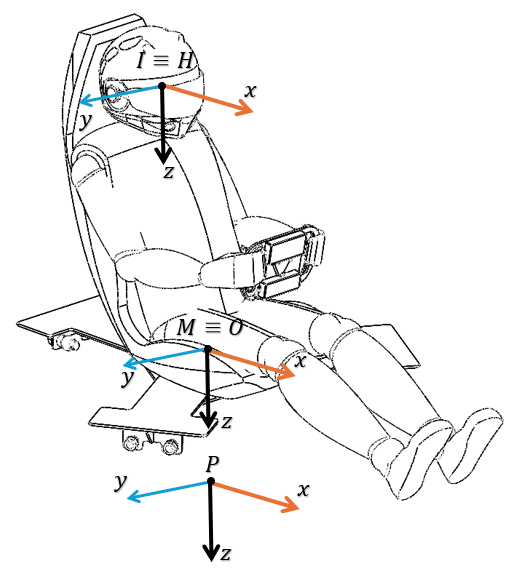
\includegraphics[width=\columnwidth]{image1.png}
  \caption{Coordinate frames and characteristic points used in the study.
           $\{O\}$: world frame fixed at platform centre at neutral
           position; $\{M\}$: moving frame attached to the platform;
           $\{H\}$: head frame; $\{I\}$: IMU frame.
           $P$: Pivot Point; $H$: head reference point; $M$: platform
           geometric centre.}
  \label{fig:frames}
\end{figure}

\subsection{Platform and Coordinate Frames}

Four coordinate frames are defined (Fig.~\ref{fig:frames}):
\begin{itemize}
  \item $\{O\}$ — world (fixed) frame, origin at the platform centre
        in the neutral position.
  \item $\{M\}$ — body frame, attached to and moving with the platform.
        At neutral, $\{M\} \equiv \{O\}$.
  \item $\{H\}$ — head frame, assumed parallel to $\{M\}$ (no relative
        rotation between head and platform body).
  \item $\{I\}$ — IMU sensor frame; misaligned with $\{M\}$ due to
        manual mounting.
\end{itemize}

Three characteristic points are defined:
$M$ (platform geometric centre),
$P$ (Pivot Point, adjustable along $Z_M$ via \texttt{centre\_z}),
and $H$ (head reference point).
The IMU is co-located with $H$, so $I \equiv H$.

\subsection{CKAS W2 Platform Parameters}

\begin{table}[!t]
  \caption{CKAS W2 Key Parameters}
  \label{tab:params}
  \centering
  \renewcommand{\arraystretch}{1.15}
  \begin{tabular}{lll}
    \toprule
    Parameter & Symbol & Value \\
    \midrule
    Base circle radius   & $r_a$   & 589.66\,mm \\
    Platform circle radius & $r_b$ & 429.57\,mm \\
    Crank arm length     & $L_1$   & 150\,mm \\
    Upper link length    & $L_2$   & 747\,mm \\
    Motor angle range    & $[\phi_\mathrm{min},\phi_\mathrm{max}]$ & $[-50°,90°]$ \\
    Nominal head height  & $H_\mathrm{head}$ & $\approx 820\mm$ \\
    \bottomrule
  \end{tabular}
\end{table}

% =========================================================================
\section{Proposed Method}
\label{sec:method}

\subsection{Kinematic Model}

For a rigid body performing pure rotation about $P$ (i.e.,
$\vv{a}_P = \vv{0}$), the acceleration at any body-fixed point $H$
is given by:
\begin{equation}
  \aH = \alp \times \rPH + \omg \times (\omg \times \rPH),
  \label{eq:rigid_body}
\end{equation}
where $\alp$ and $\omg$ are the angular acceleration and velocity
vectors expressed in $\{M\}$, and $\rPH = [r_x,\,r_y,\,r_z]^T$ is
the unknown position vector from $P$ to $H$ in $\{M\}$.

Expanding \eqref{eq:rigid_body} in component form:
\begin{equation}
  \aH = \underbrace{\begin{bmatrix}
    -(\omega_y^2+\omega_z^2) & \omega_x\omega_y - \alpha_z & \omega_x\omega_z + \alpha_y \\
    \omega_x\omega_y + \alpha_z & -(\omega_x^2+\omega_z^2) & \omega_y\omega_z - \alpha_x \\
    \omega_x\omega_z - \alpha_y & \omega_y\omega_z + \alpha_x & -(\omega_x^2+\omega_y^2)
  \end{bmatrix}}_{\mathbf{M}(t)}
  \rPH.
  \label{eq:matrix_form}
\end{equation}

\textbf{Observability.}
For a \emph{pure Roll} maneuver ($\omg = [\omega_x,0,0]^T$), the
matrix $\mathbf{M}$ has $\mathrm{rank} < 3$, so $r_x$ is unobservable.
Roll data yield $[r_y,\,r_z]$; Pitch data yield $[r_x,\,r_z]$.
Combining both maneuvers gives the full vector $\rPH$.

\subsection{Least-Squares Solver}

Stacking $n$ time samples:
\begin{equation}
  \underbrace{\begin{bmatrix} \aH^1 \\ \vdots \\ \aH^n \end{bmatrix}}_{\mathbf{A}}
  =
  \underbrace{\begin{bmatrix} \mathbf{M}^1 \\ \vdots \\ \mathbf{M}^n \end{bmatrix}}_{\mathbf{B}}
  \rPH,
  \label{eq:ls_system}
\end{equation}
the least-squares solution is:
\begin{equation}
  \rPH^* = (\mathbf{B}^T\mathbf{B})^{-1}\mathbf{B}^T\mathbf{A}.
  \label{eq:ls_solution}
\end{equation}
Because measured data contain sensor noise and processing errors,
\eqref{eq:ls_solution} minimises the residual
$\|\mathbf{B}\rPH - \mathbf{A}\|^2$.

\subsection{Signal Pre-Processing Pipeline}

\begin{figure}[!t]
  \centering
  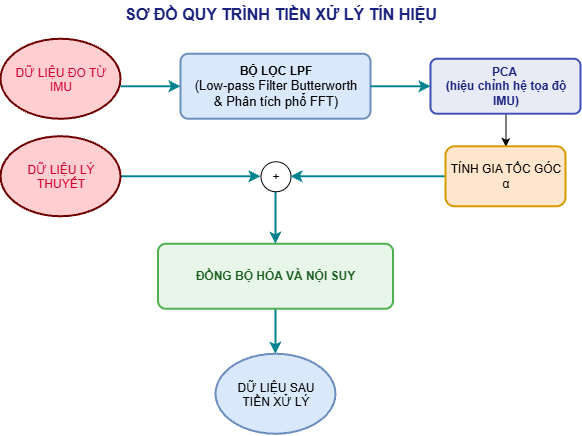
\includegraphics[width=0.9\columnwidth]{So_do_tien_xu_ly.png}
  \caption{Pre-processing pipeline: (1) FFT analysis and Butterworth LPF,
           (2) PCA-based axis alignment, (3) angular acceleration by
           numerical differentiation, (4) time synchronisation with
           simulation reference.}
  \label{fig:pipeline}
\end{figure}

The pipeline (Fig.~\ref{fig:pipeline}) consists of four steps applied
to the raw IMU output.

\subsubsection{Low-Pass Filtering}
High-frequency mechanical vibrations corrupt $\omg$, and subsequent
numerical differentiation amplifies noise by $\mathcal{O}(f^2)$.
A 2nd-order Butterworth IIR filter with zero-phase forward-backward
filtering (MATLAB \texttt{filtfilt}) is used.
The cut-off frequency $f_c = 0.5\,\mathrm{Hz}$ is selected from
FFT analysis of the steady-state signal; the dominant motion peak
at $0.25\,\mathrm{Hz}$ is preserved.

\subsubsection{PCA-Based Axis Alignment}
Manual IMU mounting introduces an unknown misalignment between $\{I\}$
and $\{M\}$, causing cross-talk (e.g., a Roll maneuver producing Pitch
$\omega_y$ readings).
The alignment rotation matrix $\mathbf{R}_{IM}$ is computed as
follows:
\begin{enumerate}
  \item \textbf{Dynamic PCA.} The principal eigenvector
        $\vv{v}_{\max}$ of the covariance matrix of filtered $\omg$
        gives the dominant motion axis.
  \item \textbf{Static gravity.} Mean linear acceleration at rest gives
        the gravity vector $\vv{g}$ in $\{I\}$.
  \item \textbf{Frame construction.}
        $\vv{\eta} = \vv{v}_{\max} \times \vv{g}$,
        $\vv{\zeta} = \vv{v}_{\max} \times \vv{\eta}$;
        columns of $\mathbf{R}_{IM}$ are the normalised
        $[\vv{v}_{\max},\,\vv{\eta},\,\vv{\zeta}]$.
\end{enumerate}
All IMU signals are transformed by $\mathbf{R}_{IM}$ before further
processing.

\subsubsection{Angular Acceleration}
Angular acceleration is obtained by central-difference differentiation
of the filtered, aligned $\omg$:
\begin{equation}
  \alp_k = \frac{\omg_{k+1} - \omg_{k-1}}{2\Delta t}.
\end{equation}

\subsubsection{Time Synchronisation}
IMU timestamps may have jitter due to microcontroller clock drift.
Linear interpolation brings IMU and simulation reference data to the
same uniform time grid before stacking \eqref{eq:ls_system}.

% =========================================================================
\section{Experimental Setup}
\label{sec:exp}

\begin{figure}[!t]
  \centering
  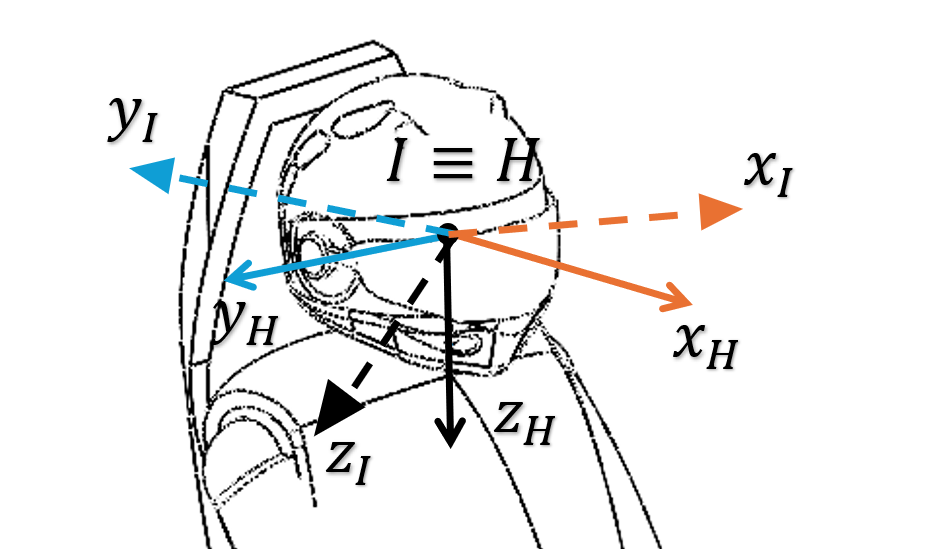
\includegraphics[width=\columnwidth]{image2.png}
  \caption{Sensor mounting and axis-alignment concept.
           Left: IMU (MW-AHRSv1) mounted at head position on the
           manikin; right: schematic showing the misalignment angle
           between $\{I\}$ and $\{M\}$ corrected by $\mathbf{R}_{IM}$.}
  \label{fig:mounting}
\end{figure}

\subsection{Hardware}

\begin{itemize}
  \item \textbf{Platform}: CKAS W2 6-RUS Gough--Stewart
        driving simulator.
  \item \textbf{IMU}: MW-AHRSv1 — provides roll/pitch/yaw angles,
        angular velocity ($\omg$) and linear acceleration ($\vv{a}$)
        at $f_s = 100\,\mathrm{Hz}$.
  \item \textbf{Reference}: 15-parameter trajectory files exported by
        \textsc{Dashboard Stewart5} (MATLAB), containing theoretical
        kinematics of the Pivot Point.
\end{itemize}

The IMU is mounted on a rigid manikin placed in the driving seat,
with measured offsets:
distance to headrest $23.13\,\text{cm}$,
distance to seat edge $23.11\,\text{cm}$,
distance to seat surface $66.67\,\text{cm}$.
These serve as a mechanical reference but are not used in the solver;
the algorithm recovers $\rPH$ solely from inertial data.

\subsection{Test Protocol}

Sinusoidal maneuvers are applied independently along Roll and Pitch axes:
\begin{itemize}
  \item Amplitude: $10°$; Frequency: $0.25\,\mathrm{Hz}$;
        Duration: $40\,\mathrm{s}$.
  \item \texttt{centre\_z} $\in \{0,-100,-200,-300,-400,-500\}\mm$.
\end{itemize}
For each setting, one Roll and one Pitch dataset is acquired, yielding
12 datasets total.
The steady-state window (excluding the first 2\,s fade-in) is used
for identification.

% =========================================================================
\section{Results}
\label{sec:results}

\subsection{Filtering and SNR Improvement}

Fig.~\ref{fig:fft} shows FFT spectra of $\alpha_x$ (Roll) and
$\alpha_y$ (Pitch) before and after Butterworth filtering.
\begin{figure}[!t]
  \centering
  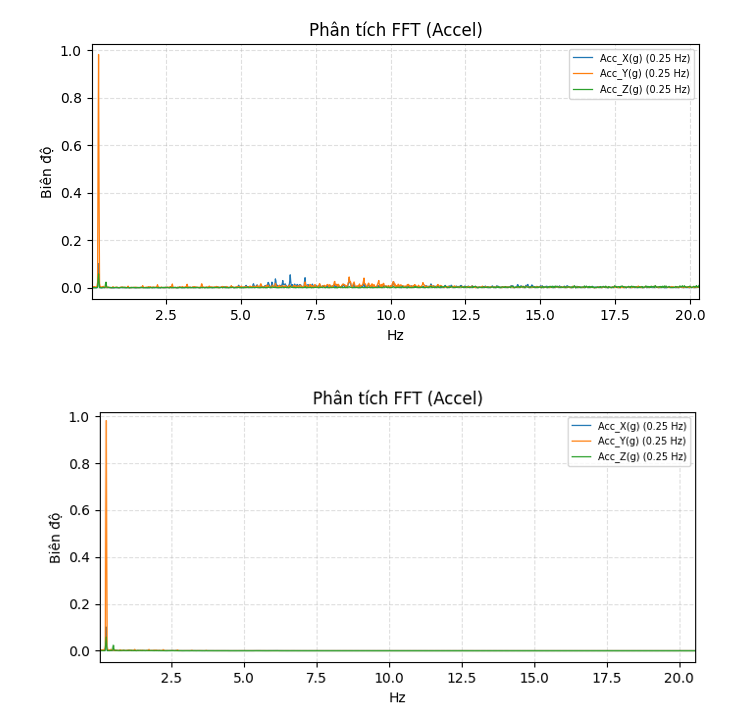
\includegraphics[width=\columnwidth]{image3.png}
  \caption{FFT spectrum and time-domain signal of angular acceleration
           before (red) and after (blue) LPF ($f_c = 0.5\,\mathrm{Hz}$,
           2nd-order Butterworth). Dominant peak at $0.25\,\mathrm{Hz}$.}
  \label{fig:fft}
\end{figure}

\noindent Before filtering:
$\mathrm{SNR}(\alpha_x) = -2.2\,\mathrm{dB}$,
$\mathrm{SNR}(\alpha_y) = -9.0\,\mathrm{dB}$ — noise dominates.
After filtering:
$\mathrm{SNR}(\alpha_x) = 32.6\,\mathrm{dB}$,
$\mathrm{SNR}(\alpha_y) = 22.4\,\mathrm{dB}$ — signal is recovered.

\subsection{PCA Axis Alignment}

Fig.~\ref{fig:pca} illustrates the cross-talk reduction.
\begin{figure}[!t]
  \centering
  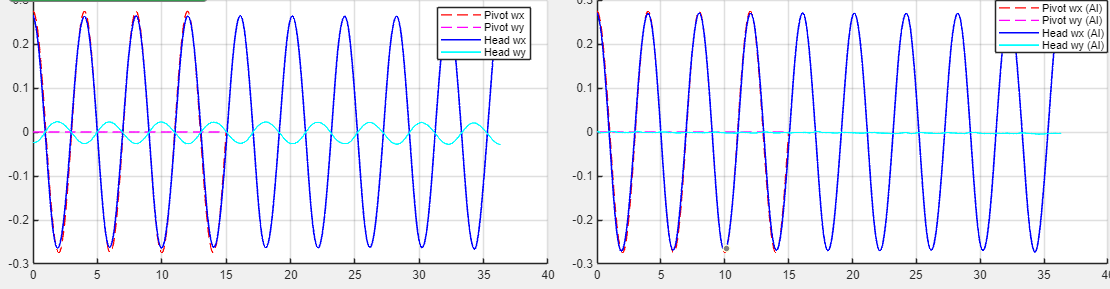
\includegraphics[width=\columnwidth]{image6.png}
  \caption{Cross-talk in $\omega_y$ during a Roll maneuver.
           Before alignment: $\omega_y / \omega_x = 9.37\,\%$.
           After PCA alignment: $\omega_y / \omega_x = 1.14\,\%$.}
  \label{fig:pca}
\end{figure}

\subsection{Identified Pivot--Head Vector}

Tables~\ref{tab:roll} and \ref{tab:pitch} list $\rPH$ results for
Roll and Pitch maneuvers respectively.
$r_{zI0}$ denotes the $Z$-component of $\rPH$ in the world frame
($r_{zI0} = r_{zI} - \texttt{centre\_z}$, accounting for the
shifted pivot origin).

\begin{table}[!t]
  \caption{Identified $\rPH$ from Roll Maneuver}
  \label{tab:roll}
  \centering
  \renewcommand{\arraystretch}{1.15}
  \begin{tabular}{rrrrrr}
    \toprule
    $c_z$ & $r_{zI}$ & $r_{yI}$ & $r_{zI0}$ & RMSE & $r_P$ \\
    (mm)  & (mm)     & (mm)     & (mm)       & (m/s²) &  \\
    \midrule
      0   & 820.7 & 33.9  & 820.7 & 0.0394 & 0.987 \\
    $-$100 & 729.1 & 28.2  & 829.1 & 0.0348 & 0.987 \\
    $-$200 & 624.6 & 31.3  & 824.6 & 0.0319 & 0.985 \\
    $-$300 & 515.6 & 22.6  & 815.6 & 0.0243 & 0.989 \\
    $-$400 & 402.1 & 19.6  & 802.1 & 0.0219 & 0.983 \\
    $-$500 & 306.3 &  7.7  & 806.3 & 0.0202 & 0.976 \\
    \midrule
    \multicolumn{3}{l}{\textbf{Mean $r_{zI0}$}} &
      \multicolumn{3}{l}{$816.4 \pm 14.3$ mm (err.\ $1.75\,\%$)} \\
    \bottomrule
  \end{tabular}
\end{table}

\begin{table}[!t]
  \caption{Identified $\rPH$ from Pitch Maneuver}
  \label{tab:pitch}
  \centering
  \renewcommand{\arraystretch}{1.15}
  \begin{tabular}{rrrrrr}
    \toprule
    $c_z$ & $r_{zI0}$ & $r_{xI}$ & $r_{zI0}$ & RMSE & $r_P$ \\
    (mm)  & (mm)      & (mm)     & (mm)       & (m/s²) &  \\
    \midrule
      0   & 821.6 & $-$313.5 & 821.6 & 0.0623 & 0.994 \\
    $-$100 & 742.2 & $-$323.4 & 842.2 & 0.0756 & 0.994 \\
    $-$200 & 603.8 & $-$289.2 & 803.8 & 0.0430 & 0.995 \\
    $-$300 & 502.7 & $-$292.6 & 802.7 & 0.0512 & 0.989 \\
    $-$400 & 403.7 & $-$292.4 & 803.7 & 0.0586 & 0.989 \\
    $-$500 & 307.3 & $-$299.9 & 807.3 & 0.0504 & 0.971 \\
    \midrule
    \multicolumn{3}{l}{\textbf{Mean $r_{zI0}$}} &
      \multicolumn{3}{l}{$813.6 \pm 28.6$ mm (err.\ $3.52\,\%$)} \\
    \bottomrule
  \end{tabular}
\end{table}

\noindent\textbf{Final identified vector.}
Combining both maneuvers:
\begin{equation}
  \rPH^* = \begin{bmatrix} -301.8 \pm 21.6 \\
                             23.9  \pm 16.2 \\
                            813.6  \pm 28.6 \end{bmatrix} \text{ mm},
  \label{eq:result}
\end{equation}
where $r_z$ is taken from Pitch (wider confidence interval, but
encompasses the Roll estimate).
The corresponding optimal \texttt{centre\_z} setting is:
\begin{equation}
  \texttt{centre\_z}^* \approx -813.6\mm.
  \label{eq:cz_result}
\end{equation}

\subsection{Acceleration Fit Quality}

Fig.~\ref{fig:accel} compares measured and model-predicted
accelerations at a representative \texttt{centre\_z} setting.

\begin{figure}[!t]
  \centering
  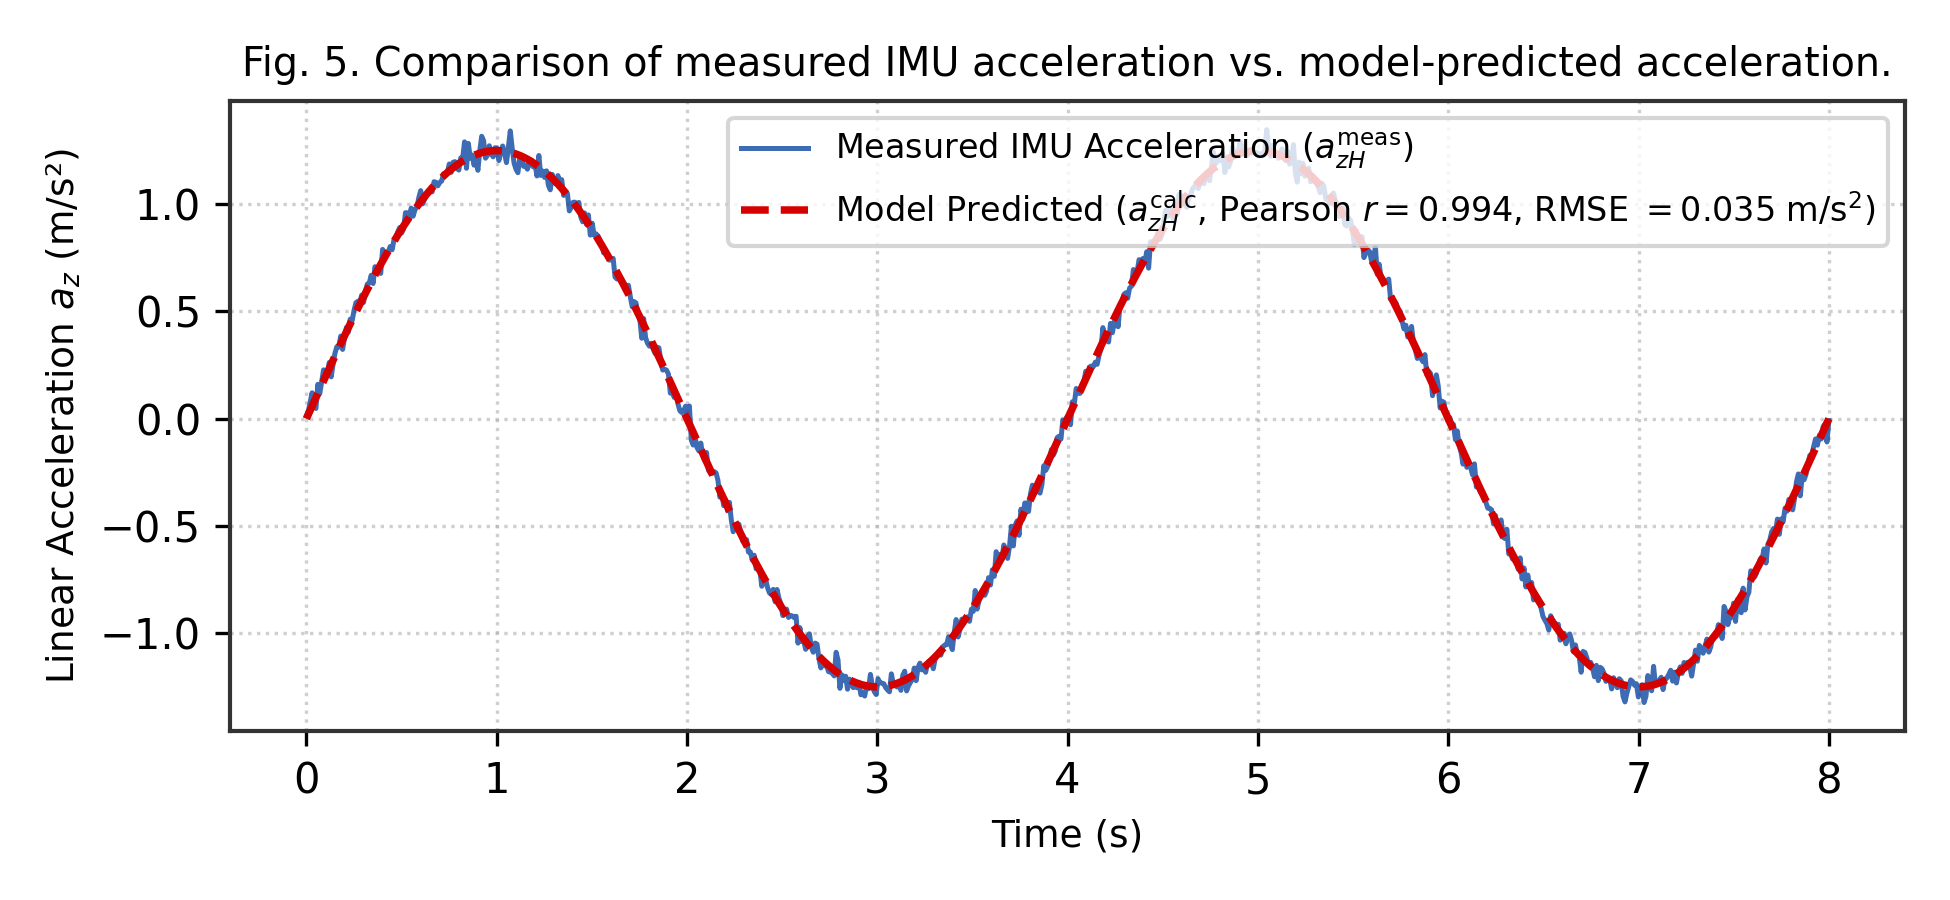
\includegraphics[width=\columnwidth]{fig5_accel_comparison.png}
  \caption{Measured (solid) vs.\ model-predicted (dashed) linear
           acceleration at the IMU / head position for Roll maneuver,
           \texttt{centre\_z} $= -400\mm$.
           Pearson $r = 0.983$, RMSE $= 0.0219\,\text{m/s}^2$.}
  \label{fig:accel}
\end{figure}

% =========================================================================
\section{Discussion}
\label{sec:discussion}

\subsection{Consistency Across Pivot Settings}

$r_{zI0}$ (the Pivot-to-Head $Z$-distance corrected for pivot offset)
remains stable across all six \texttt{centre\_z} settings in both Roll
and Pitch maneuvers (Tables~\ref{tab:roll}--\ref{tab:pitch}), with
relative errors below $4\,\%$.
This confirms that the kinematic model \eqref{eq:rigid_body} correctly
captures the geometry regardless of pivot location, and that the
pre-processing pipeline effectively removes sensor artefacts.

\subsection{Lateral Components}

The $r_{yI}$ component ($23.9 \pm 16.2\mm$, relative error
$41.8\,\%$) has a large relative uncertainty due to its small
absolute value; the absolute error ($16.2\mm$) is in fact smaller than
that of $r_{xI}$ ($21.6\mm$).
For motion-cueing purposes $r_{yI}$ is negligible compared to $r_{zI}$
and $r_{xI}$.

\subsection{Limitations}

\begin{itemize}
  \item The model assumes a rigid connection between IMU and platform
        (seat and manikin deformation neglected).
  \item Only single-axis maneuvers are used; combined DOF excitation
        could improve observability for all three components
        simultaneously.
  \item Gravity is assumed parallel to $Z_P$; inclination errors
        propagate into $\alp$ via \eqref{eq:rigid_body}.
\end{itemize}

% =========================================================================
\section{Conclusion}
\label{sec:conclusion}

This paper has presented an IMU-based method to identify the
Pivot-to-Head position vector $\rPH$ on the CKAS W2 6-RUS driving
simulator.
The approach requires only a low-cost AHRS sensor, standard sinusoidal
excitation, and a three-step pre-processing pipeline (LPF, PCA, sync)
before applying a batch least-squares solver.

Experimental results across six pivot configurations consistently
recover $r_z = 813.6 \pm 28.6\mm$ from Pitch maneuvers
and $816.4 \pm 14.3\mm$ from Roll maneuvers, with Pearson
$r \ge 0.97$ and RMSE $\le 0.076\,\text{m/s}^2$.
The identified \texttt{centre\_z}$^* \approx -813.6\mm$ can be
directly used as a motion-cueing configuration parameter.

Future work will extend the method to simultaneous multi-axis
maneuvers, online recursive identification, and compensation of seat
compliance.

% =========================================================================
\section*{Acknowledgment}
The authors thank the Smart Equipment and Robot Lab, HUST, for access
to the CKAS W2 platform.

% =========================================================================
\begin{thebibliography}{00}

\bibitem{Stewart1965}
D.~Stewart,
``A platform with six degrees of freedom,''
\emph{Proc.\ Inst.\ Mech.\ Eng.}, vol.~180, no.~1,
pp.~371--386, 1965.

\bibitem{Gough1956}
V.\,E.~Gough and S.\,G.~Whitehall,
``Universal tyre test machine,''
\emph{Proc.\ FISITA 9th Int.\ Tech.\ Congr.}, pp.~117--137, 1956.

\bibitem{Kolasinski1995}
E.\,M.~Kolasinski,
``Simulator sickness in virtual environments,''
U.S.\ Army Res.\ Lab., Tech.\ Rep.\ ARI-TR-1027, 1995.

\bibitem{Draper2001}
M.~Draper, H.~Viire, T.~Furness, and M.~Gawron,
``Effects of image scale and system time delay on simulator sickness
within head-coupled virtual environments,''
\emph{Human Factors}, vol.~43, no.~1, pp.~129--146, 2001.

\bibitem{Kalman1960}
R.\,E.~Kalman,
``A new approach to linear filtering and prediction problems,''
\emph{J.\ Basic Eng.}, vol.~82, no.~1, pp.~35--45, 1960.

\bibitem{Merlet2006}
J.-P.~Merlet,
\emph{Parallel Robots}, 2nd~ed.
Springer, 2006.

\bibitem{Dasgupta2000}
B.~Dasgupta and T.\,S.~Mruthyunjaya,
``The Stewart platform manipulator: A review,''
\emph{Mech.\ Mach.\ Theory}, vol.~35, no.~1, pp.~15--40, 2000.

\bibitem{CKASDatasheet}
CKAS Mechatronics,
``CKAS W Series Motion Platform Data Sheet,'' 2019.
[Online]. Available: \url{https://www.ckas.com.au/w-series}

\end{thebibliography}

\end{document}
